% !TeX spellcheck = en_US
\documentclass[french]{article}
\usepackage[T1]{fontenc}
\usepackage[utf8]{inputenc}
\usepackage{lmodern}
\usepackage[a4paper]{geometry}
\usepackage{babel}
\usepackage{graphicx}

\begin{document}
\title{Nuages de points et modélisation 3D\\
TP 3 : Neighborhood descriptors}
\author{Marius Dufraisse}
\date{}

\maketitle


\paragraph{Question 1.} When the radius is too big small details do not appear in the computed normal map. For instance borders of the windows can be seen when the radius is equal to 50cm (see Figure \ref{fig:q1-50cm}) but when the radius is equal to 5m the wall is in a single color (see Figure \ref{fig:q1-5m}).

When the radius is too small, noise in the data results in noise in the normal (see Figure \ref{fig:q1-5cm} for results with a 5cm radius).



\begin{figure}[h]
	\centering
	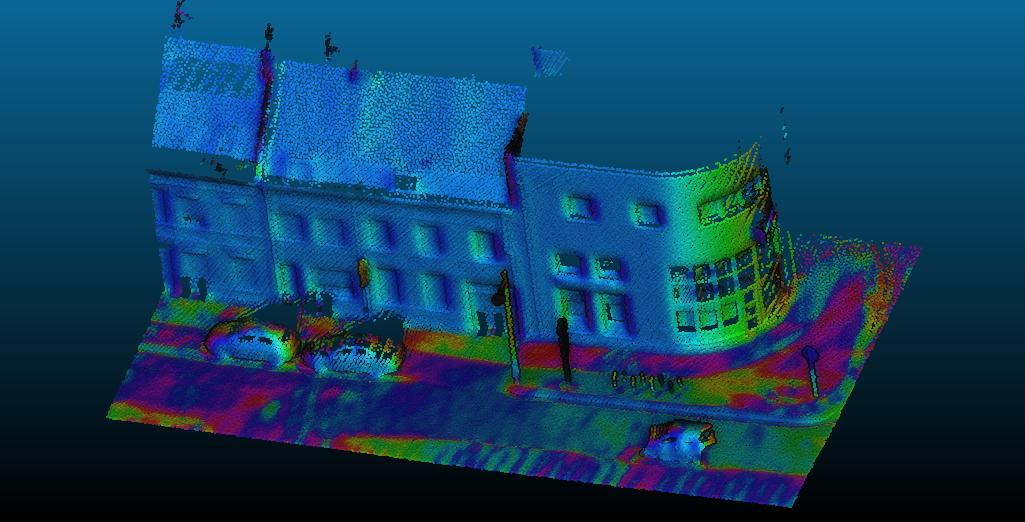
\includegraphics[width=0.6\linewidth]{q1-r50cm.jpg}
	\caption{Normals obtained with a radius of 50cm.}
	\label{fig:q1-50cm}
\end{figure}

\begin{figure}[h]
	\centering
	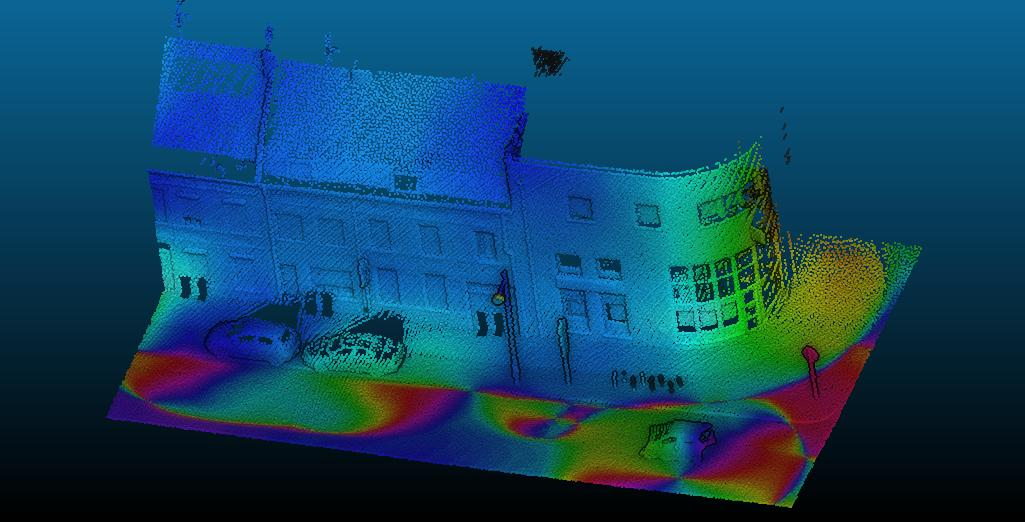
\includegraphics[width=0.6\linewidth]{q1-r5m.jpg}
	\caption{Normals obtained with a radius of 5m.}
	\label{fig:q1-5m}
\end{figure}

\begin{figure}[h]
	\centering
	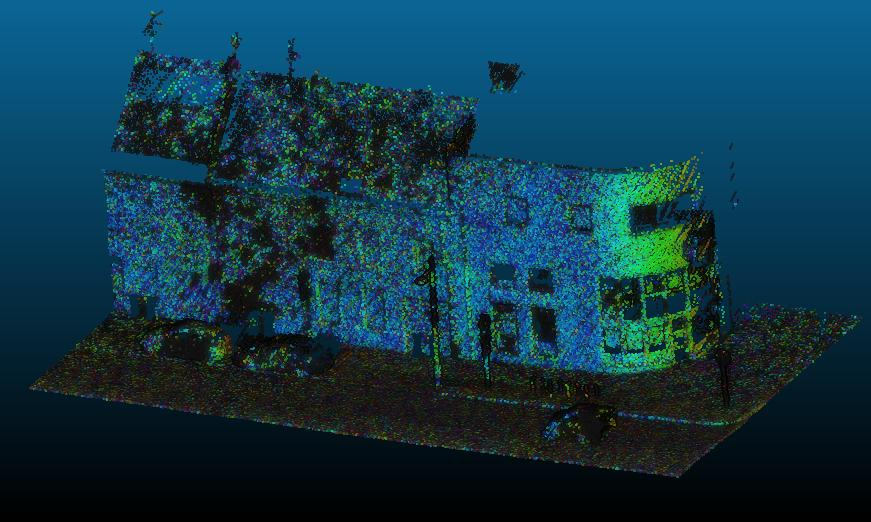
\includegraphics[width=0.6\linewidth]{q1-r5cm.jpg}
	\caption{Normals obtained with a radius of 5cm.}
	\label{fig:q1-5cm}
\end{figure}

\paragraph{Question 2.} A good way to choose the radius would be to take it as small as the biggest detail we want to analyze. However, I have no idea how this could be computed using just the point cloud.

\paragraph{Question 3.} My results are shown in Figure \ref{fig:q3}. In order to have normal oriented in the same direction I compared the computed normal direction to a fixed vector. This was not enough to get normals from every part of the image in the same direction : CloudCompare provides algorithms that solved this issue.

\begin{figure}[h]
	\centering
	\begin{minipage}{0.49\linewidth}
		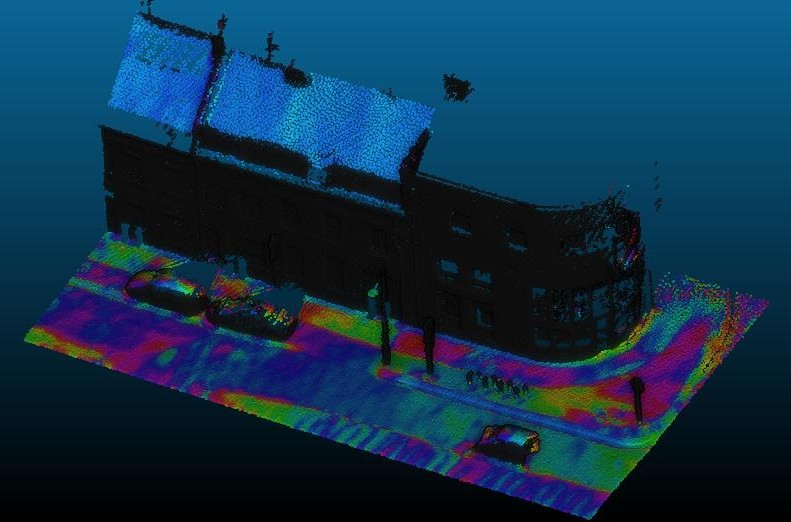
\includegraphics[width=\linewidth]{q3-raw.jpg}
	\end{minipage}\hfill
	\begin{minipage}{0.49\linewidth}
		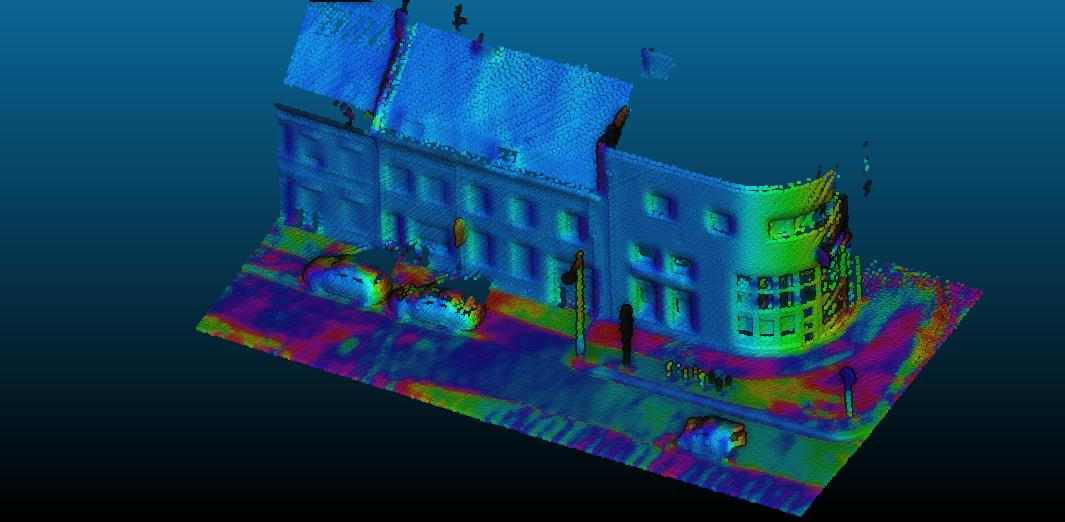
\includegraphics[width=\linewidth]{q3-cheat.jpg}
	\end{minipage}
	\caption{On the left, the normal converted to dip I obtained when trying to align them with a reference vector. On the right, the same normals only using ClouCompare to orient them.}
	\label{fig:q3}
\end{figure}


\end{document}
